%%
%% Mise en Place for Agentic Coding
%% VibeX 2026 - Positioning Paper
%%
\documentclass[sigconf]{acmart}

%% Bibliography style
\bibliographystyle{ACM-Reference-Format}

%% Conference metadata
\acmConference[VibeX 2026]{1st International Workshop on Vibe Coding and Vibe Researching}{9--12 June, 2026}{Glasgow, Scotland, United Kingdom}

%% Remove ACM-specific fields for workshop submission
\settopmatter{printacmref=false}
\renewcommand\footnotetextcopyrightpermission[1]{}
\pagestyle{plain}

%% Packages
\usepackage{booktabs}
\usepackage{tikz}
\usetikzlibrary{arrows.meta,positioning,shapes.geometric,fit,backgrounds}

%% Title
\title{Mise en Place for Agentic Coding: Deliberate Preparation as Context Engineering Methodology}

%% Authors
\author{Andrew Zigler}
\email{andrew.zigler@linearb.io}
\orcid{0009-0001-8073-5917}
\affiliation{%
  \institution{LinearB}
  \city{Los Angeles}
  \country{USA}
}

\begin{document}

%% Abstract
\begin{abstract}
The rapid adoption of AI coding agents has produced a dominant workflow pattern --- often called ``vibe coding'' --- that prioritizes speed of implementation over deliberate preparation. We argue that this approach creates a systematic alignment problem: agents that lack sufficient context produce code requiring extensive debugging and refactoring, consuming substantial development time. Drawing on the culinary concept of \emph{mise en place} (everything in its place; abbreviated MEP), we propose a three-phase preparation methodology for agentic coding: (1) contextual grounding, where domain expertise and tacit knowledge are externalized into structured documents; (2) collaborative specification, where human-agent dialogue produces detailed design artifacts; and (3) task decomposition, where specifications are converted into structured, dependency-aware task records. We report on the application of MEP during a competitive hackathon, where roughly two hours of preparation enabled a rapid parallel implementation of a full-stack educational platform by concurrent AI agents. We introduce the concept of \emph{context fluency} as an emerging developer skill --- the ability to create rich, structured context that agents can act on --- and connect it to established frameworks in backward design and tacit knowledge externalization. We conclude with a research agenda for empirically validating preparation-phase methodologies in AI-assisted software development.
\end{abstract}

%% CCS Concepts
\begin{CCSXML}
<ccs2012>
   <concept>
       <concept_id>10011007.10011074</concept_id>
       <concept_desc>Software and its engineering~Software creation and management</concept_desc>
       <concept_significance>500</concept_significance>
   </concept>
   <concept>
       <concept_id>10011007.10011074.10011099</concept_id>
       <concept_desc>Software and its engineering~Collaboration in software development</concept_desc>
       <concept_significance>500</concept_significance>
   </concept>
   <concept>
       <concept_id>10003120.10003121</concept_id>
       <concept_desc>Human-centered computing~Human computer interaction (HCI)</concept_desc>
       <concept_significance>300</concept_significance>
   </concept>
</ccs2012>
\end{CCSXML}

\ccsdesc[500]{Software and its engineering~Software creation and management}
\ccsdesc[500]{Software and its engineering~Collaboration in software development}
\ccsdesc[300]{Human-centered computing~Human computer interaction (HCI)}

%% Keywords
\keywords{agentic coding, mise en place, context engineering, vibe coding, context fluency}

\maketitle

%% Sections
\section{Introduction}

AI coding agents are remarkably capable at code generation: controlled
studies of GitHub Copilot report productivity gains of 21--55\% across
programming tasks~\cite{peng2023copilot}, and the broader ecosystem can
now scaffold entire applications from natural-language descriptions.
Yet the dominant workflow pattern---what
Karpathy~\cite{karpathy2025vibe} termed ``vibe coding''---prioritizes
speed of implementation over deliberate preparation. The developer
describes an intent, the agent produces code, and misalignments are
resolved through iterative correction. This creates a systematic
alignment problem: agents operating without sufficient context produce
code that requires extensive rework. Veracode reports that 45\% of
AI-generated code contains security flaws~\cite{veracode2025ai}, and
practitioners consistently observe that debugging misaligned agent
output can consume substantial development
time~\cite{huntley2025ralph, yegge2025beads}. The bottleneck in agentic
coding is not code generation but \emph{alignment} between developer
intent and agent output---specification compliance, architectural
fidelity, and low corrective-commit ratios.

We argue that this alignment problem is fundamentally a \emph{preparation}
problem. Drawing on the culinary concept of \emph{mise en place} (MEP)---a
French term meaning ``everything in its place''---we propose a
preparation-first methodology for agentic coding. In professional kitchens,
thorough preparation enables fluid execution: every ingredient is
measured and every tool positioned so that once cooking begins, the
chef's hands never pause to search. The same principle applies to agent
orchestration. When domain expertise, design intent, and task boundaries
are externalized into structured artifacts \emph{before} agents begin
writing code, the resulting implementation is more aligned, more
coherent, and less costly to verify. MEP formalizes this preparation
into three steps: contextual grounding (tacit knowledge captured in
machine-legible documents), collaborative specification (human-agent
dialogue producing detailed design artifacts), and task decomposition
(specifications converted into dependency-aware work records). We
position MEP relative to spec-driven development, prompt engineering,
and iterative AI coding in Section~\ref{sec:related}.

This paper makes four contributions:
\begin{enumerate}
  \item A three-phase MEP methodology for agentic coding, grounded
    in backward design~\cite{wiggins1998understanding} and tacit knowledge
    externalization~\cite{polanyi1966tacit}.
  \item A case study applying this methodology in a competitive hackathon,
    with quantitative data on preparation artifacts and implementation
    outcomes.
  \item The concept of \emph{context fluency} as an emerging developer
    skill---the ability to create rich, structured context that AI agents can
    act on.
  \item A research agenda with five open questions for empirical validation
    of preparation-phase methodologies.
\end{enumerate}

\section{Background and Related Work}
% TODO: Content to be written by writing agents
% Target: ~600 words
%
% Key points to cover:
% - AI-assisted coding workflows: Copilot studies, productivity gains,
%   security concerns (Veracode 45% flaw rate)
% - Emerging preparation methodologies: RPI (Horthy), Spec-Driven
%   Development (GitHub Spec Kit), Context Engineering (Anthropic/Gartner)
% - Practitioner innovations: Ralph Loop (Huntley), Beads (Yegge),
%   beads_rust (Emanuel)
% - Theoretical foundations: Backward design (Wiggins & McTighe),
%   tacit knowledge (Polanyi)
% - Gap: No formalized, theoretically-grounded methodology for
%   preparation-phase work
\lipsum[2-3]

\section{The Mise en Place Methodology}
\label{sec:methodology}

We propose \emph{mise en place} as a structured preparation methodology for agentic coding.
The term, borrowed from professional culinary practice, describes the discipline of
arranging every ingredient and tool before cooking begins. In a professional kitchen,
the speed of service is a direct function of the thoroughness of preparation:
chefs who invest time in mise en place execute complex dishes fluidly, while
those who skip preparation spend service time searching, measuring, and
recovering from avoidable errors. We observe an analogous dynamic in
AI-assisted software development:
when practitioners invest in deliberate preparation---externalizing domain knowledge,
producing detailed specifications, and decomposing work into structured task
records---the resulting agent execution is faster, more aligned with intent, and
requires less corrective iteration.

The methodology formalizes preparation into three sequential phases, each
producing defined artifacts that feed into the next. Following the backward design
principle~\cite{wiggins1998understanding}, the phases are completed before any
implementation begins. Figure~\ref{fig:methodology}
illustrates the three phases and their relationship to agent execution.

\begin{figure}[t]
  \centering
  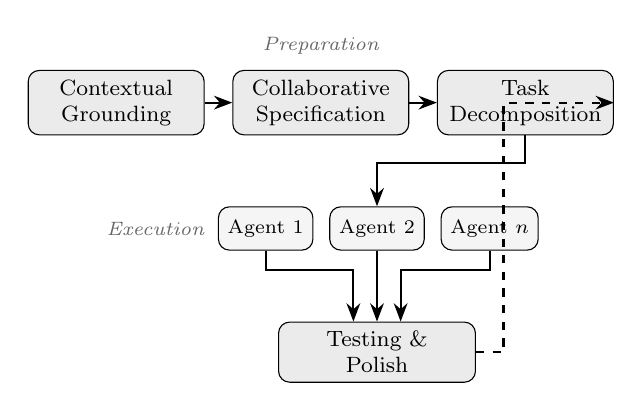
\begin{tikzpicture}[
    >=Stealth,
    phase/.style={draw, rounded corners, fill=black!8, minimum width=2.1cm,
      minimum height=0.7cm, font=\footnotesize, align=center, text width=2cm},
    agent/.style={draw, rounded corners, fill=black!4, minimum width=1.2cm,
      minimum height=0.55cm, font=\scriptsize, align=center},
    label/.style={font=\scriptsize\itshape, text=black!60},
    arw/.style={->, thick},
  ]
    % Preparation phases
    \node[phase] (p1) {Contextual\\Grounding};
    \node[phase, right=0.35cm of p1] (p2) {Collaborative\\Specification};
    \node[phase, right=0.35cm of p2] (p3) {Task\\Decomposition};

    % Arrows between phases
    \draw[arw] (p1) -- (p2);
    \draw[arw] (p2) -- (p3);

    % Parallel agents
    \node[agent, below=0.9cm of p2, xshift=-0.7cm] (a1) {Agent 1};
    \node[agent, right=0.2cm of a1] (a2) {Agent 2};
    \node[agent, right=0.2cm of a2] (a3) {Agent $n$};

    % Arrow from decomposition to agents
    \draw[arw] (p3.south) -- ++(0,-0.35) -| (a2.north);

    % Testing node
    \node[phase, below=0.9cm of a2, minimum width=2.5cm] (test) {Testing \&\\Polish};

    % Arrows from agents to testing
    \draw[arw] (a1.south) -- ++(0,-0.25) -| ([xshift=-0.3cm]test.north);
    \draw[arw] (a2.south) -- (test.north);
    \draw[arw] (a3.south) -- ++(0,-0.25) -| ([xshift=0.3cm]test.north);

    % Feedback loop
    \draw[arw, dashed] (test.east) -- ++(0.35,0) |- (p3.east);

    % Labels
    \node[label, above=0.08cm of p2] {Preparation};
    \node[label, left=0.05cm of a1] {Execution};

  \end{tikzpicture}
  \caption{The mise en place methodology: three preparation phases produce structured context that enables parallel agent execution with minimal coordination overhead. Dashed arrow indicates a feedback loop for defects.}
  \label{fig:methodology}
\end{figure}

\subsection{Phase 1: Contextual Grounding}

The first phase externalizes domain expertise and tacit knowledge into structured
documents that agents can consume. Its purpose is to capture context that agents
cannot generate independently---what Polanyi~\cite{polanyi1966tacit} characterized
as tacit knowledge, the understanding that practitioners possess but struggle
to articulate. In agentic coding, this includes institutional context,
domain-specific constraints, competitive landscape awareness, design philosophy,
and the practitioner's accumulated judgment about what constitutes quality in
the target domain.

The artifacts produced are briefing documents: markdown files encoding domain
knowledge, competitive analysis, architectural preferences, and design philosophy.
These documents serve a dual purpose. First, they force the practitioner to
articulate knowledge that would otherwise remain implicit. Second, they create a
persistent context layer that agents reference throughout implementation, reducing
the need for repeated clarification. Following backward
design~\cite{wiggins1998understanding}, contextual grounding begins with outcomes
(the ``why'') rather than technical features (the ``what''), establishing alignment
criteria that propagate through subsequent phases.

\subsection{Phase 2: Collaborative Specification}

The second phase produces detailed design artifacts through structured
human-agent dialogue. The practitioner describes intent; the agent proposes
implementation details; the practitioner accepts, rejects, or modifies the
proposal. This iterative refinement continues until both parties converge on a
specification detailed enough for implementation without further clarification.

The key mechanism is the encoding of value judgments as specification constraints.
What to \emph{exclude} is as important as what to include. Scope
management---the deliberate decision to constrain features, simplify interactions,
or defer capabilities---represents a class of judgment that agents cannot make
independently. The output is a comprehensive design document that specifies
screens, interactions, data flows, and quality standards, capturing not just the
\emph{what} but the \emph{why} behind each decision. This distinction separates
collaborative specification from conventional requirements gathering: the
specification encodes rationale, enabling agents to make aligned micro-decisions
during implementation without escalating to the practitioner.

\subsection{Phase 3: Task Decomposition}

The final preparatory phase converts the specification into structured,
dependency-aware task records. We use
Beads~\cite{yegge2025beads, emanuel2025beadsrust}---lightweight, Git-backed
JSON records with priorities, dependencies, and acceptance criteria---though
the principle applies to any structured task tracking system.

Fine-grained decomposition enables parallel agent execution without coordination
overhead. When each task is independently executable---with clear boundaries,
defined inputs and outputs, and explicit dependencies---multiple agents can work
simultaneously. The coordination burden shifts from runtime (agents negotiating)
to preparation time (the practitioner defining task boundaries), where human
judgment about system architecture is most valuable. The output of this phase is a dependency graph where each node represents an
independently executable unit of work. The graph structure enables the
practitioner to identify the critical path, allocate agents to parallelizable
tasks, and monitor progress through structured completion signals. It also
provides a natural mechanism for prioritization: core features are
executed first, while stretch goals are explicitly deferred, preventing scope
creep during implementation.

The three phases of mise en place draw individually on established work---tacit
knowledge externalization~\cite{polanyi1958personal}, the RPI
methodology~\cite{horthy2025rpi}, and iterative task
delegation~\cite{huntley2025ralph}. The methodology's contribution is their
integration into a sequential, phase-gated process with defined artifacts and
theoretical grounding in backward design: the insistence that all three phases
complete before implementation begins.

\section{Case Study: Competitive Hackathon}
\label{sec:casestudy}

We report on the application of MEP during a competitive hackathon
to illustrate the methodology's behavior under realistic constraints. The
setting imposed fixed time limits, external evaluation, and a requirement to
produce working software---conditions that favor rapid iteration and
penalize unproductive preparation.

\subsection{Setting}

The hackathon took place in January 2026, organized around a publisher's
editorial archive and an AI-powered content API. Approximately 12 teams
competed in a five-hour window to build working prototypes, with judging
by an industry panel and a \$5{,}000 prize for the top project. Teams
self-organized around pitches submitted before the event~\cite{event2026hackathon}.
The practitioner-researcher had professional backgrounds in both
education and software engineering, a combination that informed the
product concept and design decisions throughout the event.

\subsection{Preparation Phase}

While most teams began coding within the first fifteen minutes, the
practitioner-researcher spent approximately two hours in deliberate
preparation, applying the three phases described in
Section~\ref{sec:methodology}.

\textbf{Contextual grounding} produced 10 planning documents totaling 9,386
words, including API exploration notes, competitive analysis, and---critically---an
extended dictation on pedagogical design philosophy drawn from the practitioner's
teaching experience, encoding tacit knowledge about how effective learning
environments create conditions for student thinking~\cite{polanyi1966tacit}.

\textbf{Collaborative specification} occurred concurrently, as the practitioner
refined the product concept through dialogue with an AI agent. The resulting
specification described a platform where teachers curate bounded research
environments from The Atlantic's archive and students conduct research using a
Socratic AI tutor. Key value judgments encoded in the specification included
constraining the product to a single assignment type (prioritizing depth over
breadth for a three-minute demo),
insisting on real API data rather than mocks, and scoping the analytics dashboard
to show the student's research \emph{journey} rather than only the final submission.

\textbf{Task decomposition} converted the specification into 64 structured
task records with priorities and dependencies. The planning-to-code
ratio---9,386 words of planning against 8,496 lines of source code---was
1.10:1. Table~\ref{tab:timeline} summarizes the timeline alongside the
deployment commit cadence.

\begin{table}[t]
  \centering
  \caption{Hackathon timeline, artifacts, and deployment cadence. Phases
    overlap inside the preparation block; agent implementation runs in
    parallel across four agents. The deployment-and-polish window
    produces nine commits at $\sim$5~minute mean intervals.}
  \label{tab:timeline}
  \footnotesize
  \begin{tabular}{@{}lrl@{}}
    \toprule
    \textbf{Phase} & \textbf{Duration} & \textbf{Key Artifacts / Cadence} \\
    \midrule
    Contextual grounding   & $\sim$2 hr      & 10 docs (9,386 words) \\
    Collab.\ specification & (concurrent)    & Product specification \\
    Task decomposition     & (concurrent)    & 64 beads w/ dependencies \\
    Agent implementation   & 184 min         & 43 beads closed (med.\ 5.9 min) \\
    \midrule
    Deploy: setup        & 22:24--22:39    & 5 commits, 1 every 3 min \\
    Deploy: gap          & 22:39--22:49    & --- \\
    Deploy: content fixes & 22:49--23:17    & 4 commits, 1 every 7 min \\
    \bottomrule
  \end{tabular}
\end{table}

\subsection{Implementation and Results}

Four parallel subagents were deployed across distinct feature areas:
classroom creation, student research workspace, day-one/\allowbreak
day-thirty demo toggle, and Socratic AI tutor. The agents drew on the
contextual grounding documents and specification produced during
preparation. The 64 task records served as the interface between
preparation and execution (Figure~\ref{fig:methodology}); each bead
encoded an independently executable unit with boundaries that required
no inter-agent coordination. Closure timestamps confirm genuine
parallelism: agents completed work simultaneously across feature
areas, with a median closure time of 5.9~minutes per bead
(Figure~\ref{fig:beadtimes}). The subsequent deployment phase produced
9~commits over 52~minutes. The final codebase comprised 43
TypeScript/TSX files totaling 8,496 lines, deployed to production as a
full-stack educational platform.

\begin{figure}[t]
  \centering
  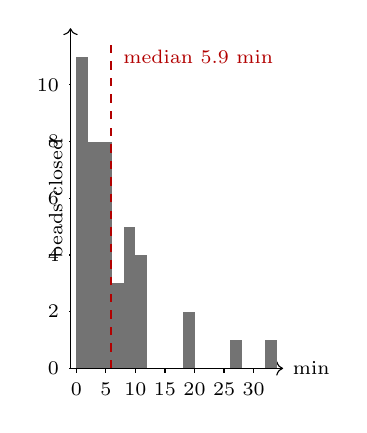
\begin{tikzpicture}[
    yscale=0.36, xscale=0.075,
    every node/.style={font=\scriptsize},
  ]
    %% Axes
    \draw[->] (-1,0) -- (35,0) node[right, font=\scriptsize] {min};
    \draw[->] (-1,0) -- (-1,12);
    %% x ticks
    \foreach \x in {0,5,10,15,20,25,30}
      \draw (\x,0) -- (\x,-0.18) node[below, font=\scriptsize] {\x};
    %% y ticks (counts)
    \foreach \y/\lab in {0/0,2/2,4/4,6/6,8/8,10/10}
      \draw (-1,\y) -- (-1.3,\y) node[left, font=\scriptsize] {\lab};
    %% Histogram bars: 2-min bins of closure times for n=43 beads
    %% Bins (lower, count): [0,2):11, [2,4):8, [4,6):8, [6,8):3,
    %%   [8,10):5, [10,12):4, [12,14):0, [14,16):0, [16,18):0,
    %%   [18,20):2, [20,22):0, [22,24):0, [24,26):0, [26,28):1,
    %%   [28,30):0, [30,32):0, [32,34):1
    \fill[black!55] (0,0)  rectangle (2,11);
    \fill[black!55] (2,0)  rectangle (4,8);
    \fill[black!55] (4,0)  rectangle (6,8);
    \fill[black!55] (6,0)  rectangle (8,3);
    \fill[black!55] (8,0)  rectangle (10,5);
    \fill[black!55] (10,0) rectangle (12,4);
    \fill[black!55] (18,0) rectangle (20,2);
    \fill[black!55] (26,0) rectangle (28,1);
    \fill[black!55] (32,0) rectangle (34,1);
    %% median line
    \draw[dashed, thick, red!70!black] (5.9,0) -- (5.9,11.6);
    \node[red!70!black, anchor=west, font=\scriptsize] at (6.3,11) {median 5.9 min};
    %% y label
    \node[rotate=90, font=\scriptsize] at (-3.5,6) {beads closed};
  \end{tikzpicture}
  \caption{Per-bead completion time distribution across the 43 closed
    hackathon beads. Most work units complete inside a single 10-minute
    agent session; long-tail outliers correspond to API-client and
    state-persistence tasks executed in parallel with shorter
    decomposed work.}
  \label{fig:beadtimes}
\end{figure}

Three observations bear on evaluation. First, the architecture required no
structural refactoring during deployment: the bugs that emerged were
integration and styling issues (API content truncation, inter-component
data flow, favicon configuration), not architectural misalignment.
Second, the preparation-to-execution ratio was approximately 5.7:1
(two hours of preparation against $\sim$21 minutes of active
implementation per agent across four parallel agents). Bug-type beads
resolved at a median 1.2~minutes (mean 1.5~min) versus 9.7~minutes for
implementation tasks, suggesting parallel-execution defects were
detected and corrected quickly.
Third, near-zero architectural rework is consistent with the hypothesis
that rich upfront context reduces agent misalignment, though we cannot
establish causation from a single case study.

\subsection{Variation Across Teams}
\label{sec:teamvariation}

The 12-team field offers a qualitative sketch of how peers approached
the same constraints. We did not instrument other teams; identities are
anonymized and observations are coarse-grained, drawing on publicly
shared pitches and event observation. Table~\ref{tab:teams} groups
pitches into thematic clusters with each team's described workflow style.

\begin{table}[t]
  \centering
  \caption{Twelve-team field at the hackathon, grouped by problem
    cluster, with workflow style as inferred from pitches and
    observation. Identifiers are anonymized; ``vibe'' denotes a
    self-described non-technical or iterative-prompting workflow,
    ``decomp.'' denotes explicit planning before coding, and ``mixed''
    denotes both modes within one team.}
  \label{tab:teams}
  \scriptsize
  \begin{tabular}{@{}p{0.06\columnwidth}p{0.46\columnwidth}p{0.16\columnwidth}p{0.12\columnwidth}@{}}
    \toprule
    \textbf{ID} & \textbf{Pitch theme} & \textbf{Cluster} & \textbf{Workflow} \\
    \midrule
    T1  & Infinite-canvas archive graph        & Discovery       & decomp.\ \\
    T2  & Reading-comprehension overlay        & Education       & vibe \\
    T3  & In-article excerpt exploration       & Discovery       & mixed \\
    T4  & AI ``knowledge gauge'' (reading level) & Accessibility & vibe \\
    T5  & Auto-generated event timelines       & Context         & vibe \\
    T6  & Topic-following / catch-up alerts    & Personalization & mixed \\
    T7  & Editorial content optimization (CORE) & Personalization & decomp.\ \\
    T8  & Reader-interpretation probes         & Trust           & decomp.\ \\
    T9  & Structured reader-expert input       & Trust           & decomp.\ \\
    T10 & Argument-evolution interaction layer & Discovery       & decomp.\ \\
    T11 & Newsroom knowledge-graph copilot     & Productivity    & decomp.\ \\
    T12 & Curated classroom research workspace (this study) & Education & decomp.\ \\
    \bottomrule
  \end{tabular}
\end{table}

Three patterns emerge. \textbf{Workflow style} split roughly in half:
teams whose pitch flagged a non-technical author or vibe-coding intent
(T2, T4, T5) leaned on iterative prompting, while engineering-led teams
(T1, T7--T12) opened with explicit planning artifacts before
generating code. \textbf{Single- versus multi-agent} use trended toward
single-agent loops; only T12 (this study) explicitly fanned out
parallel subagents from a decomposed plan. \textbf{Artifact production}
was correspondingly uneven: vibe-leaning teams presented working
surfaces with limited written specification, whereas
decomposition-leaning teams produced design notes shared with judges.
We cannot link these patterns to outcome quality without controlled
comparison, but the field reads as a natural sample of the
preparation-versus-iteration spectrum that motivates RQ1 and the
multi-team replication study in Section~\ref{sec:agenda}.

\section{Context Fluency: An Emerging Skill}

Effective agentic coding requires a skill set distinct from both
traditional programming and prompt engineering. We propose
\emph{context fluency} to describe this capability: the ability to
create rich, structured context that AI agents can act on. Context
fluency captures domain expertise, value judgments, and design intent
in machine-legible form---not as one-shot prompts, but as persistent
informational environments. Prompt engineering optimizes individual
instructions; context fluency is \emph{upstream} of prompting,
concerned with the informational architecture surrounding agent
execution~\cite{anthropic2025context, gartner2025context}. Where MEP
describes a sequence of phases producing artifacts, context fluency
describes the practitioner skill that makes the process effective.

We identify four components of context fluency:
\begin{description}
  \item[Decomposition:] Breaking problems into discrete, parallelizable
    tasks with clear boundaries, enabling concurrent agent execution.
  \item[Specification:] Describing not just \emph{what} to build but
    \emph{why}, so agents can make aligned micro-decisions without human
    intervention.
  \item[Constraint definition:] Knowing what to exclude, simplify, or
    defer---scope management as a first-class concern.
  \item[Domain encoding:] Externalizing tacit
    knowledge~\cite{polanyi1966tacit} that agents cannot generate on
    their own---directly instantiating what Nonaka and
    Takeuchi~\cite{nonaka1995knowledge} term \emph{externalization},
    converting tacit knowledge into explicit, communicable form.
    Twenty minutes of dictated pedagogical intuitions
    produced context that substantially reduced iteration on the
    domain-specific tutor component.
\end{description}

These components map to established frameworks. Backward
design~\cite{wiggins1998understanding} contributes outcome-driven
preparation; Polanyi's tacit knowledge~\cite{polanyi1958personal}
frames the externalization challenge---``we know more than we can
tell,'' and context fluency is the discipline of telling it anyway.
Context fluency also resembles pedagogical scaffolding: structuring
an environment so the learner (or agent) can act independently.

If context fluency is a distinct skill, the implications extend
beyond individual practice. For developer education, curricula should
cultivate specification, decomposition, and domain-encoding alongside
programming competencies. For hiring, practitioners with strong
domain knowledge and pedagogical instincts may be disproportionately
effective in agentic workflows~\cite{dakhel2025humanai}. For tool
design, preparation aids---task systems~\cite{yegge2025beads,
emanuel2025beadsrust}, specification frameworks~\cite{github2025speckit},
and context engineering platforms~\cite{anthropic2025context}---are
essential infrastructure, not optional enhancements.

\section{Research Agenda and Conclusion}

\subsection{Research Agenda}

Mise en place as described here rests on a single case study and conceptual
argument. Empirical validation across practitioners, domains, and agent
models is essential. We propose five research questions to guide this work:

\begin{description}
  \item[RQ1:] \emph{Does deliberate preparation reduce agent misalignment
    compared to iterative development, and at what cost-benefit threshold?}
    Controlled experiments comparing preparation-first and iteration-first
    workflows on equivalent tasks could establish whether the upfront time
    investment yields net savings---and identify the project characteristics
    where each approach dominates.

  \item[RQ2:] \emph{What constitutes ``sufficient'' context for agentic
    work---can we define stopping criteria for the preparation phase?}
    A saturation-style analysis of context documents, measuring alignment
    quality as a function of context volume and specificity, would help
    practitioners know when to stop preparing and start building.

  \item[RQ3:] \emph{How does context fluency vary across practitioners,
    domains, and agent models?} Studies comparing developers with different
    backgrounds (e.g., education, domain expertise, years of experience) on
    identical agentic tasks could reveal whether context fluency is a
    trainable skill or a function of prior domain
    knowledge~\cite{polanyi1958personal}.

  \item[RQ4:] \emph{Can mise en place principles scale beyond prototyping to
    sustained, multi-month development projects?} Our hackathon case
    represents a constrained, time-limited setting. Longitudinal case studies
    tracking preparation practices and their outcomes across full product
    development cycles would test the methodology's applicability at
    scale~\cite{dakhel2025humanai}.

  \item[RQ5:] \emph{What is the relationship between preparation time and
    implementation quality across different project complexities?} A
    multi-project dataset correlating preparation artifacts (document count,
    word count, task granularity) with implementation metrics (defect rate,
    alignment accuracy, rework ratio) could yield quantitative models of the
    preparation-quality relationship~\cite{alomar2025promptware}.
\end{description}

These questions span experimental, observational, and longitudinal designs.
We believe the most immediately tractable is RQ1, which could be addressed
with paired tasks and a modest participant pool.

\subsection{Conclusion}

Mise en place is not a finished methodology but a starting framework---a
formalization of preparation practices that experienced practitioners are
already converging on independently~\cite{huntley2025ralph, horthy2025rpi,
yegge2025beads}. Our single case study suggests that deliberate preparation
can dramatically compress implementation time and reduce architectural
misalignment, but we make no claim of generalizability from one hackathon.
What we do claim is that the alignment problem in agentic coding is
fundamentally a preparation problem, and that the field would benefit from
treating the work that happens \emph{before} agents write code as a
first-class engineering discipline.

The concept of context fluency offers a lens for understanding emerging
practitioner skills in AI-assisted development---skills that bridge domain
expertise, pedagogical design, and specification craft. We invite empirical
validation, replication across domains and practitioner profiles, and the
development of tools that support preparation-phase
work~\cite{anthropic2025context, github2025speckit}. The code, increasingly,
is the easy part. The hard part---knowing what to build and
why---remains a distinctly human contribution.


%% References
\bibliography{references}

\end{document}
